
\chapter{QUADRO METODOLÓGICO}
\par O quadro metodológico é a descrição dos passos realizados para a 
execução do trabalho. Serão listados, nos tópicos a seguir, os itens essenciais
no desenvolvimento do trabalho, sendo eles as técnicas, procedimentos, práticas e instrumentos
utilizados, o contexto de aplicação e o tipo de pesquisa utilizado que será apresentado no tópico a seguir.

\section{Tipo de pesquisa}

\par Será explicado, nesta sessão, o tipo de pesquisa escolhido para nortear o
desenvolvimento deste trabalho, justificando também como ele se enquadra no tipo
escolhido.

\par Para \citeonline[p.42]{pesquisa_social_gil}, a pesquisa tem um caráter
pragmático, é um “processo formal e sistemático de desenvolvimento do método científico. 
O objetivo fundamental da pesquisa é descobrir respostas para problemas mediante
o emprego de procedimentos científicos”.

\par Este trabalho terá como base a metodologia de pesquisa aplicada, pois
será desenvolvida uma aplicação inteligente utilizando Algoritmos Genéticos para
o auxílio na tomada de decisão sobre o processo de produção de calças de uma
confecção. Esta pesquisa consiste em procurar respostas para problemas propostos
baseados em padrões e conhecimentos já existentes.

\par \citeonline[p.35]{livro_metodos_de_pesquisa} afirmam que o método de
pesquisa aplicada, "objetiva gerar conhecimentos para aplicação prática, dirigidos a
solução de problemas específicos. Envolve verdades e interesses locais."  

\par Segundo \citeonline{livro_metodologia_de_estudo_de_pesquisa}, a pesquisa
aplicada tem como motivação básica a solução de problemas
concretos, práticos e operacionais e também pode ser chamada de pesquisa
empírica pois o pesquisador precisa ir a campo, conversar com pessoas e
presenciar relações sociais.

\par Como citam \citeonline{tecnicas_de_pesquisa}, a pesquisa aplicada
caracteriza-se por possuir um interesse prático, quando os resultados serão aplicados ou utilizados na
solução de problemas que ocorrem na realidade, sempre visando gerar conhecimento
para solucionar situações específicas.

\par Como já foi explicado o tipo de pesquisa em que se enquadra este trabalho,
ela deve ser aplicada a um determinado contexto, conforme será explicado no
tópico a seguir.

\section{Contexto de pesquisa}

\par Sabe-se que com a alta competitividade no mercado, as empresas, cada vez mais,
buscam diferenciais competitivos para seus produtos e, neste cenário, a ideia
de redução de custos se torna essencial, uma vez que tal redução pode ser
refletida no preço dos produtos permitindo que estes se diferenciem. Dentre
os fatores que viabilizam tais reduções está a otimização de processos que
consistem em organizar os procedimentos relacionados à produção de forma que
estes se tornem mais eficazes.

\par O software desenvolvido neste trabalho visa organizar uma linha de produção
de forma que esta se torne o mais eficiente possível. Será utilizada como
base uma fábrica de confecção de calças situada na cidade de
Cachoeira de Minas - MG, porém a base de conhecimento pode ser aplicada a outros
tipos de negócios que seguem o mesmo padrão de desenvolvimento de produtos.

\par Como cada funcionário da fábrica citada trabalha em sua casa, é preciso ter
uma boa forma de distribuir a produção para que o transporte da matéria-prima
seja eficaz, trazendo para a empresa uma redução de custos e um tempo de
produção menor.
Para isso, é necessário que o software conheça os procedimentos de
produção da fábrica, como seus funcionários trabalham e se estão sendo alocados
de forma correta. A aplicação cruza todas essas informações gerando para o
usuário uma relação de como ele deve distribuir a matéria-prima para produção
das peças.

\par Como cada funcionário trabalha em sua casa é preciso saber qual a
melhor rota para se entregar a matéria-prima ou recolher o que foi produzido
para que seja passado para a próxima etapa da produção. O software avalia a
melhor rota levando em consideração as peças que precisam ser produzidas, as
habilidades de cada funcionário e se os mesmos não estão alocados em outros
processos de produção. Analisando esses fatos, o software sabe a melhor forma
para distribuição da produção e os funcionários tem suas tarefas distribuídas
de forma a se obter o menor tempo e o  menor custo de produção.


\section{Instrumentos}

\par Segundo \citeonline{aula_joelma_26_03_15}, instrumentos de pesquisa são a
forma pela qual os dados são coletados para a realização do trabalho, podendo ser,
dentre outras, por meio de reuniões, questionários e entrevistas. Para
este projeto utilizaremos os instrumentos descritos nas subseções a seguir.

\subsection{Entrevistas}
\par Segundo \citeonline{metodoliga_qualitativas_na_sociologia}, entrevista é
uma interação entre duas pessoas em que uma representa o entrevistador, 
que através de perguntas, obtêm informações por parte de outra pessoa que
representa o entrevistado.


% entrevista é um
% “processo de interação social entre duas pessoas na qual uma delas, o entrevistador,
% tem por objetivo a obtenção de informações por parte do outro, o entrevistado”



\par Foi realizada uma entrevista com o dono da empresa de confecção com o
objetivo de entender seu modelo de negócio para que então fosse possível começar
a fazer o levantamento dos requisitos do sistema. Para
\citeonline[p.128]{pressman2011engenharia}, levantamento de requisitos de
software consiste em

\begin{citacao}
perguntar ao cliente, aos usuários e aos demais interessados quais são os
objetivos para o sistema ou produto, o que deve ser alcançado, como o sistema ou
produto atenda às necessidades da empresa e, por fim, como o sistema ou produto
deve ser utilizado no dia a dia.
\end{citacao} 

\par A entrevista ocorreu no dia 09/05/2015 para conhecer mais sobre o processo de 
produção da fábrica. Nesta entrevista ficou esclarecido todo processo e também se teve 
acesso à forma como era controlada a distribuição da produção entre os funcionários. Toda
produção era controlada por meio de planilhas Excel que eram
controladas e alimentadas pelo proprietário. Tais planilhas contemplavam as
estimativas de produção, as datas de entrega de lotes de peças encomendado,
levando em consideração a quantidade de peças, o corte e também o tempo em que cada peça levaria
para ser entregue.


\subsection{Reuniões}
\par De acordo com \citeonline{ref_reuniao}, reunião é o ajuntamento de
pessoas para se tratar de um determinado assunto em que é necessário que se
tenha conclusões sobre as questões que foram discutidas.

\par Durante o desenvolvimento do projeto seriam realizadas várias reuniões
com o proprietário da fábrica de calças para saneamento de dúvidas, sugestões e
outros assuntos que poderiam surgir. Todavia foi realizada apenas uma reunião com o proprietário
da empresa para poder entender como funciona o processo de produção, pois foi constatado nesta reunião que o
processo de produção foi alterado. No processo inicial, o qual foi a base para este projeto, cada funcionário trabalhava em
sua residência e as peças eram distribuídas entre eles. Atualmente o processo
passou por muitas mudanças, uma delas é que a produção é feita em um lugar
somente sem a necessidade de transportar as peças entre as casas dos
funcionários. Segundo o proprietário isso gerou um ganho de tempo bem expressivo
pois as peças circulavam dentro de um mesmo local e não pela cidade. 

\par Considerando essa mudança, não foram feita outras reuniões com o proprietário da fábrica
pois o projeto em pesquisa não atende mais o processo de produção atual da fábrica, porém o
projeto pode ser usado em outras empresas que seguem a forma de produção que foi
pesquisado. Assim, com ajuda do professor Roberto, nosso orientador, foi definido 
um escopo para o desenvolvimento da aplicação baseando-se no processo inicial da
fábrica de calças, que se resume em construir uma aplicação levando em consideração que:

\begin{itemize}
	
	\item O processo de desenvolvimento das calças deveria ser dividido em atividades com 
	ordem de precedência;
	
	\item cada atividade poderia ser feita por uma ou mais costureiras, de acordo com a habilidade de cada uma;
	
	\item cada costureira gasta um tempo, medido em segundos, para fabricar uma peça;
	
	\item O usuário deveria ser capaz de cadastrar um novo processo, costureiras e habilidades;
	
	\item O total de peças deveria ser dividido em lotes e cada costureira deveria receber uma quantidade de lote
	distribuída aleatoriamente;
	
	\item O software deveria então oferecer como saída a melhor distribuição de forma a se produzir no menor tempo,
	considerando o tempo de produção de cada costureira e o transporte das peças entre elas.
	
\end{itemize}

\par A sessão a seguir descreve como foi realizado cada item do escopo demonstrado acima.



\section{Procedimentos}

\par Esta sessão descreve os procedimentos realizados na execução do projeto.

\subsubsection{Framework de desenvolvimento}
\par Primeiramente é necessário ressaltar que, para o desenvolvimento da aplicação, foi utilizada uma base desenvolvida pelo professor Artur Barbosa durante as aulas de sistemas especialistas, do VII período do curso de sistemas de informação nesta universidade.
Esta base também denominada \textit{framework}, define regras a serem seguidas no desenvolvimento de cada elemento
de um algorítimo genético. Este \textit{framework} é definido dentro da seguinte estrutura:

\begin{itemize}
	
	\item Classe \texttt{GAModel}:
	\par A classe \texttt{GAModel} é basicamente a classe mãe de todos os elementos de um algoritmo genético, 
	ela representa o modelo que irá armazenar a população de indivíduos além de ser a classe que armazena os 
	parâmetros que definem as configurações do algoritmo, tais como, tipo de cruzamento, tipo de mutação, 
	tamanho da população etc.
	
	\par A classe contém os seguintes atributos:
	
	\begin{itemize} 
		\item \textit{populationSize}:
		Este atributo define qual será o tamanho da população, ou seja, quantos indivíduos irão formar cada população;
		
		\item \textit{generationQuantity}:
		Como já explicado anteriormente, o processo de cruzamento e mutação se repete até que o número de indivíduos, 
		definido no atributo anterior, seja atingido formando assim uma nova população e então, por sua vez, 
		este processo de geração de novas populações se repete até que seja atingido um número de gerações definido 
		pelo programador. Este atributo representa esta quantidade;
		
		\item{elitism}:
		Atributo do tipo \textit{boolean} que representa se o algoritmo vai ter a função de elitismo. 
		Esta função, como já foi explicado anteriormente, quando está ativada (com valor \textit{true}), 
		no momento de começar a se criar uma nova população os dois melhores indivíduos da população que será 
		substituída já começam a fazer parte da nova população, antes de começar o processo de cruzamento e mutação. 
		Este mecanismo garante que a nova população terá pelo dois indivíduos iguais ao da antiga população, o que irá 
		impedir que a nova população seja pior que a primeira;
		
		\item{foreignIndividualRate}:
		
		
		\item{mutationRate}:
		Como descrito no quadro teórico, a mutação é o fato de realizar pequenas alterações no indivíduo a fim de que 
		este possa se tornar ainda melhor. Este parâmetro define uma porcentagem, geralmente baixa, que define quando 
		o indivíduo sofrerá mutação ou não. Esta questão ficará mais claras mais abaixo, quando será explicado o passo 
		a passo da execução do algoritmo.
		
		\item{mutationQuantity}:
		Caso a mutação for ocorrer para o indivíduo, a alteração aleatória será feita nos cromossomos. 
		Este parâmetro define quantos cromossomos do indivíduo deve ser alterado pela mutação;
		
		\item{selectionType}:
		Conforme descrito no quadro teórico, existem várias formas de seleção dos indivíduos para realizarem 
		o cruzamento. Este parâmetro define qual será a forma escolhida pelo programador ao implementar o seu problema. 
		No \textit{framework} este parâmetro é do tipo \texttt{enum} e pode assumir 2 valores o \textit{ROULETTE}, 
		que representa o método roleta e o \textit{CLASSIFICATION}, que representa o método de classificação;
		
		\item{crossType}:
		Assim como a seleção, existe diversas formas de fazer o cruzamento dos indivíduos. Este atributo, 
		também do tipo \texttt{enum} representa a forma de cruzamento e pode receber os valores \textit{Binary}, 
		\textit{Permutation}, \textit{Uniform} e \textit{Aritmetic};
		
		\item{mutationType}:
		Segue as mesma forma que o selectionType e o crossType e pode assumir os valores \textit{Permutation}, 
		\textit{Binary} e \textit{Numerical}.
		
	\end{itemize}
	
	\item Classe \texttt{Individual}:
	\par A classe abstrata \texttt{Individual}, encontra-se dentro do pacote edu.univas.edu.tcc.gacore e  
	representa a estrutura básica de um indivíduo. A classe contém uma \texttt{lista} do tipo 
	\texttt{Cromossomo}, que será descrito mais abaixo, que contém uma coleção de objetos que representam as 
	características da solução.
	
	\par A Classe contém ainda um atributo chamado \texttt{valor} que irá armazenar a qualidade, ou seja, qual é o custo
	da solução representada pelo indivíduo, tal valor é recebido no retorno da operação calcularValor() descrita abaixo.
	
	\par Com relação as operações, além dos \textit{getters and setters} e o construtor, que recebe a lista 
	de cromossomos como parâmetro, a classe contém a operação abstrata \texttt{calcularValor()}, esta operação é 
	quem realiza a função de avaliação, explicada anteriormente, que mede a qualidade do indivíduo. 
	Desta forma, ao utilizar este \textit{framework}, a classe que representa o indivíduo do problema deve herdar 
	desta classe  \texttt{Individual}. Fazendo isso tal classe passará a ter uma lista de cromossomos e o atributo 
	que representa o seu valor e a classe obrigatoriamente terá que implementar a operação 
	\texttt{calcularValor()}, já que esta é abstrata na classe mãe, permitindo assim que o programador 
	desenvolva a função de avaliação específica para o seu problema.
	
	\item Classe \texttt{Chromosome}:
	\par É uma classe abstrata, que possui todos os métodos abstratos, desta forma
	ela só existe para garantir que os cromossomos do problema irão implementar os
	métodos necessários para o funcionamento do algoritmos. Estes métodos são:
	
	\begin{itemize}
		
		\item \texttt{equals}: Necessário para efeito de comparação dos cromossomos;
		
		\item \texttt{doMutation}: Este é o método que realiza a mutação. Este deve
		ser implementado pela classe que representa o cromossomo, pois a
		mutação é feita a nível deste.
		
		\item \texttt{clone}: Este método devolve um objeto exatamente com os mesmos
		atributos do objeto, porém com instâncias diferentes.
		
	\end{itemize}
	
	
	\item Classe \texttt{IndividualPair}:
	\par A classe \texttt{IndvidualPair} possui uma estrutura simples. Apenas
	represnta dois indivíduos. Ela se torna necessária, pois o processo de
	cruzamento dos indivíduos retornam dois novos indivíduos, desta forma, como 
	no Java não é possível retornar dois valores, é retornado então um objeto desta
	classe contendo os dois novos indivíduos criados. 
	
	
	\item Classe \texttt{GAController}:
	\par A classe \texttt{GAController}, como o própio nome já diz, é o
	controlador de todo processo de excução do algoritmo genético.
	Ela recebe no seu construtor o modelo que é do tipo \texttt{GAModel}, que como
	já explicado anteriormente, armazena os parâmetros a serem seguidos na
	execução do algoritmo. Além disso, através do seu principal método
	denomidado \texttt{execute}, ela é responsável por criar novas populações, a
	partir de cruzamentos, mutações, elitismo e etc, tendo também a
	repsonsabilidade de chamar a função de classificação e avaliação de cada indivíduo.
	
	\par Os pontos a seguir descrevem basicamente os passos executados dentro do
	método \texttt{execute}. Mais detalhes serão vistos mais a frente quando será
	descrito a implementação do algoritmo da fábrica de calças, pois será necessário 
	realizar algumas adaptações neste framework.
	
	\begin{itemize}
		\item	Criação da população inicial, através do método createInitialPopulation
		do objeto da classe model;
		
		\item Classificação e avaliação da população inicial através do método
		\texttt{classify};
		
		\item Realização do processo de elitismo, através do método
		\texttt{doElitism};
		
		\item Inserção de indivíduos estrangeiros na população;
		
		\item Realização do processo de seleção de indivíduos, atrvés do método
		\texttt{doSelection};
		
		\item Execução do processo de cruzamento e mutação, através do método
		\texttt{doCrossing} e \texttt{doMutaion} respectivamente.
		
		
	\end{itemize}
	
	\par Após os passos citados acima, uma nova população foi criada e está
	armazenada na variável \texttt{newGeneration}, assim o método
	\texttt{setPopulation} do objeto \texttt{model} é chamado para então substituir
	a antiga população pela nova. Como a execução está dentro de uma estrutura de repetição
	\texttt{FOR}, o algoritmo volta ao início desta e recomeça o processo de
	criação de uma outra população. Este processo para quando o número de gerações, 
	definido no parâmetro \texttt{getGenerationQuantity} do objeto \texttt{model}
	for atingido, neste caso é dado o comando \texttt{break} e o \texttt{loop} é encerrado.
	% 	Para começar é chamado o método  \texttt{createInitialPopulation} da classe
	% 	\texttt{GAModel} para criar a população de indivíduos, este método será
	% 	implementado pela classe que irá herdar da classe \texttt{GAModel}.
	
	% 	\par Cada indivíduo representa uma solução para o problema, sua estrutura é
	% 	composta pela parte da calça a ser produzida, a costureira com
	% 	habilidade para produzir essa peça e o numero de lotes sorteados a ela.
	% 	Para explicar melhor precisa-se produzir um lote de 500 peças, será preciso
	% 	produzir 500 partes da frente, 500 partes de traz, etc., e assim
	% 	sucessivamente.
	% 	Esse lote de 500 peças é divdido entre os indivíduos da população. Para um
	% 	melhor entender a estrutura de um indivíduo veja a figura 5 a seguir:
	% 	
	% 	\begin{figure}[h!]
	% 	\centerline{\includegraphics[scale=0.5]{./imagens/individuos.png}}
	% 	\caption[Representação da estrura de um indivíduo]
	% 	{Representação da estrura de um indivíduo \textbf{Fonte:} Desenvolvido pelos autores}
	% 	\label{fig:exemplo1}
	% 	\end{figure} 
	
	
	
\end{itemize}

A Figura X representa o diagrama de classes que demonstra a estrutura em questão.
(Desenhar diagrama de classe do framework no ASTAH)

\par Posterior a definição das regras de desenvolvimento, os próximos tópicos apresentam a implementação 
dos elementos do algoritmo genético, seguindo as definições do \textit{framework}.

\subsection{Representação do processo de produção}

\par Primeiramente foi definido como seria o processo de fabricação. Este foi pensado com base no 
processo da fábrica, em que a confecção das peças deveriam ser divididas em atividades que representam
cada parte da calça. Neste contexto, surgiu a necessidade de determinar uma ordem para a execução do processo, 
devido ao fato de que algumas atividades dependem da finalização de outras para poderem ser
realizadas. A Figura X demonstra basicamente um exemplo de ordem de execução do processo de confecção.

\begin{figure}[h!]
	\centerline{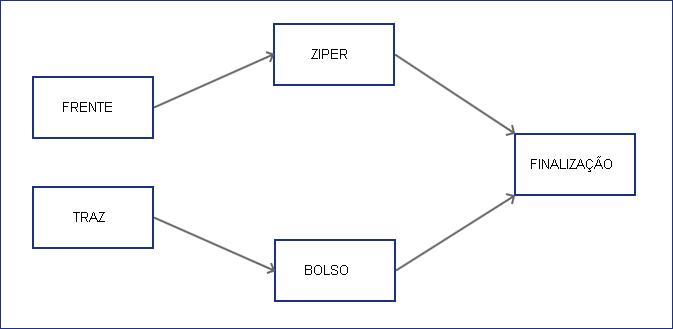
\includegraphics[scale=0.6]{./imagens/processo1.png}}
	\caption[Processo de fabricação]
	{Demonstração de um processo de fabricação \textbf{Fonte:} Desenvolvido pelos autores}
	\label{fig:exemplo1}
\end{figure}

\par Para representar este processo e suas atividades no software, foram utilizadas tabelas do banco de dados, conforme
mostra a Figura X.

\begin{figure}[h!]
	\centerline{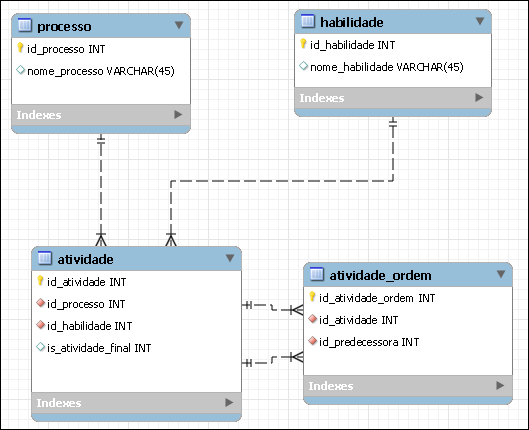
\includegraphics[scale=0.7]{./imagens/representacao_processo.png}}
	\caption[Processo de fabricação]
	{Representação do processo de fabricação no banco de dados \textbf{Fonte:} Desenvolvido pelos autores}
	\label{fig:exemplo1}
\end{figure}

\par A tabela \texttt{processo} tem como finalidade gerar um código único para representar 
cada processo, pois cada modelo de calça possui um processo diferente que pode possuir atividades
diferentes que são representadas na tabela \texttt{atividade} onde é feita a relação que define quais são
as atividades de um processo,  além de conter quais são as habilidades necessárias para cada atividade, ou seja, cada registro desta 
tabela representa uma atividade do processo e qual habilidade é necessária para sua execução. O campo 
\texttt{is-atividade-inicial}, quando tem o valor 1, define que tal atividade é a última do processo, 
tomando como base a Figura X, ela seria a atividade de Finalização. Esta \textit{flag} é importante no momento de 
calcular o tempo total de execução do processo e será vista com mais detalhes posteriormente, e, por fim, a tabela 
\texttt{atividade-ordem} é onde é feita a definição de ordem de execução das atividades.


\subsection{Distribuição das atividades (População inicial, cruzamento e mutação)}
\par Com relação a distribuição das atividades, foi definido que o total de peças a ser produzido deveria ser
dividido em lotes e então em cada atividade este número de lote deveria ser distribuído entre as costureiras que
possuem a habilidade em questão. Por exemplo: se a quantidade total de peças de uma ordem de produção for 500,
primeiramente deve-se definir qual será o número de peças por lote, neste caso, se for definido que cada lote  
deverá ter 50 peças, então o resultado final será 500/50 ou seja 10 lotes contendo 50 calças cada um. Neste sentido, seguindo
o exemplo apresentado  na Figura X, a distribuição deverá ser feita de forma que para cada atividade do processo seja distribuído
o trabalho de 10 lotes, ou seja, 10 lotes da parte da frente deve ser confeccionado e enviados para as costureiras que sabem colocar
o zíper e posteriormente estas enviam os 10 lotes para as costureiras que fazem finalização. Estas últimas irão depender
também de 10 lotes da parte de trás que também devem passar pelas costureiras que fazem a confecção dos bolsos. 


\par Com base nesses requisitos, um dos papeis desempenhado pelo algoritmo genético está na distribuição de
trabalho descrita acima. O algoritmo irá distribuir, de forma aleatória, o número de lotes definido entre as costureiras
de cada atividade, conforme mostra a figura X. 

\begin{figure}[h!]
	\centerline{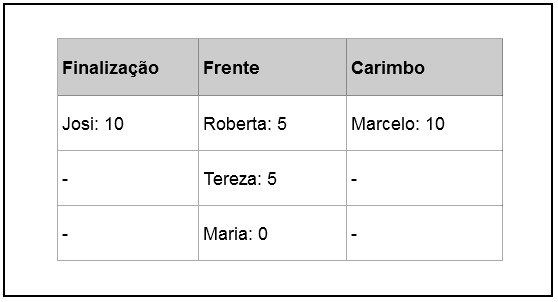
\includegraphics[scale=1.0]{./imagens/distribuicao_exemplo.png}}
	\caption[Distribuição de trabalho]
	{Exemplo de distribuição de lotes para as costureiras \textbf{Fonte:} Desenvolvido pelos autores}
	\label{fig:exemplo1}
\end{figure}

\par Como já explanado no quadro teórico, a estrutura do algoritmo genético é composta
por populações que são formadas por indivíduos que por sua vez são formados por cromossomos.
Cada indivíduo representa uma solução e cada cromossomo do indivíduo representa uma de suas características. 
Assim então é gerado uma população inicial de indivíduos e, a partir desta, um processo de cruzamento 
e mutação é iniciado a fim de que possa ser gerados novos indivíduos que representem soluções ainda melhores 
que seus antecessores.

\par Neste sentido, para a realização do algoritmo de distribuição de lotes, o processo de definição indivíduo
foi o primeiro passo do desenvolvimento da aplicação. Isso se deu devido ao fato de que o indivíduo é a parte 
crucial para que se possa definir a lógica a ser seguida para a definição da população inicial, o tipo de cruzamento 
a função de avaliação etc. Neste caso, cada indivíduo da população irá representar uma forma de distribuir as atividades e
cada número de lotes distribuído a determinada costureira irá representar um cromossomo. Tomando como base o exemplo da 
Figura X, o quadro, como um todo, representa o indivíduo e cada distribuição, como por exemplo Frente= Marta: 5, representa 
um cromossomo.

\par Para fazer esta representação em Java, primeiramente foi criado uma classe denominada \texttt{ProcessoChromosome} e
é representada no diagrama abaixo:

\begin{figure}[h!]
	\centerline{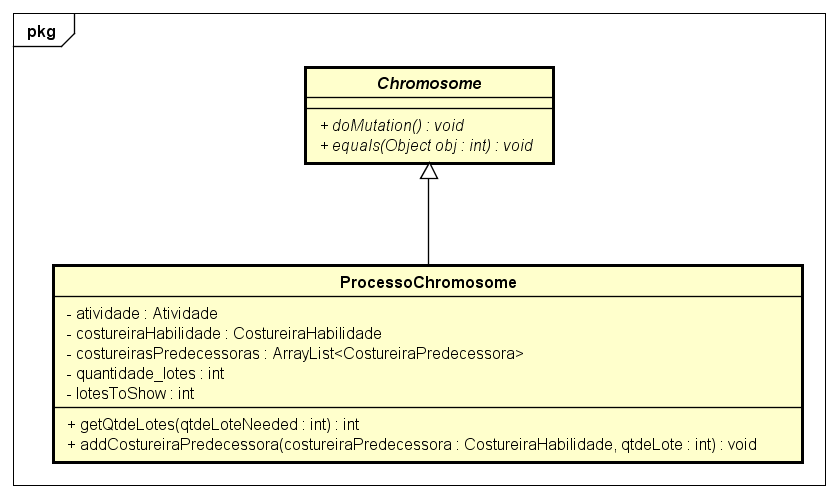
\includegraphics[scale=0.6]{./imagens/processo_chromosome_diagram.png}}
	\caption[ProcessoChromosome Class]
	{Classe ProcessoChromosome \textbf{Fonte:} Desenvolvido pelos autores}
	\label{fig:exemplo1}
\end{figure}


\par A classe \texttt{ProcessoChromosome} herda de \texttt{Chromosome} do \textit{framework} descrito acima. Por enquanto
é necessário compreender apenas os atributos \texttt{atividade}, \texttt{costureiraHabilidade} e \texttt{quantidade-lotes}, 
que recebem seus valores por um construtor, os demais atributos e métodos são utilizados pela função de avaliação e serão 
explicados mais adiante. O atributo atividade é do tipo \texttt{int} e representa o \texttt{ID} da atividade a qual se está
atribuindo a costureira e a quantidade de lotes, este identificador vem do banco de dados e será passado na criação do cromossomo
sempre que for necessário se criar um indivíduo. O atributo costureiraHabilidade é do tipo CostureiraHabilidade. Esta classe
é o mapeamento da tabela costureira-habilidade do banco de dados, esta tabela faz a relação entre quais habilidades cada costureira
possuem e quanto tempo esta gasta para fazer uma peça de cada parte, conforme demonstra a figura X.


\begin{figure}[h!]
	\centerline{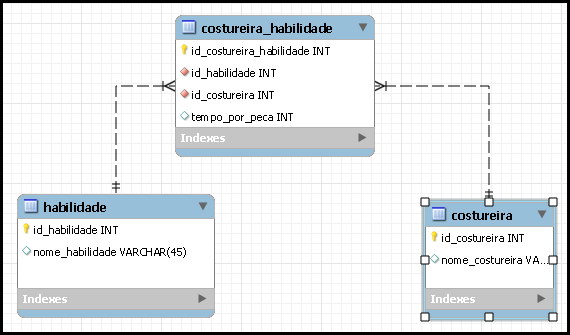
\includegraphics[scale=0.9]{./imagens/costureira_habilidade_tabela.png}}
	\caption[Tabela costureira-habilidade]
	{Armazenamento de dados das costureiras \textbf{Fonte:} Desenvolvido pelos autores}
	\label{fig:exemplo1}
\end{figure}


\par A classe \texttt{CostureiraHabilidade}, conforme demonstrada na Figura X, possui um atributo habilidade do mesmo tipo do nome, 
outro que representa a costureira e um terceiro para representar o tempo que tal costureira casta para confeccionar uma peça de tal
habilidade. Fez-se necessário ter um atributo da classe CostrutiraHabilidade ao invés de simplesmente ter um objeto do tipo Costureira
pois na função de avaliação, como será visto mais adiante, é necessário se ter o tempo que a costureira gasta para fazer a peça e este
tempo pode variar para uma mesma costureira que tem diferentes habilidades. 


\begin{figure}[h!]
	\centerline{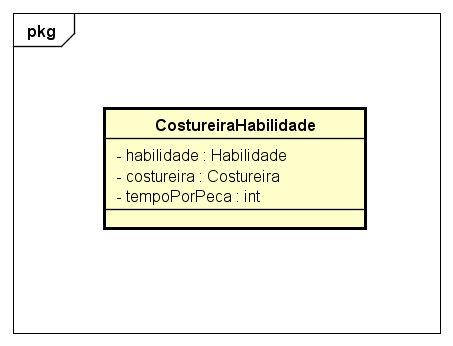
\includegraphics[scale=0.9]{./imagens/costureiraHabilidade_class.png}}
	\caption[Classe CostureiraHabilidade]
	{Classe CostureiraHabilidade \textbf{Fonte:} Desenvolvido pelos autores}
	\label{fig:exemplo1}
\end{figure}


 \par Assim, para representar cada característica da solução, tomando como exemplo a Figura X(quadro), 
o fato de Marta fazer 5 lotes da parte da frente é representado no Java criando se um objeto da classe \texttt{ProcessoCromosomo}
passando no construtor o \texttt{id} da atividade Frente, um objeto de costureiraHabilidade, cujo atributo \texttt{costureira} represente
a Marta e o atributo \texttt{habilidade} à habilidade em questão e a quantidade de lote que esta deverá confeccionar, que seria, neste caso, 5.
 
\par 






\par Cada costureira sabe fazer uma ou mais partes da calça e gasta um determinado tempo, medido em segundos, que
varia de acordo com a habilidade, conforme demonstrado na Figura X. Além disso existe um tempo de percurso entre 
cada costureira. 

\begin{figure}[h!]
	\centerline{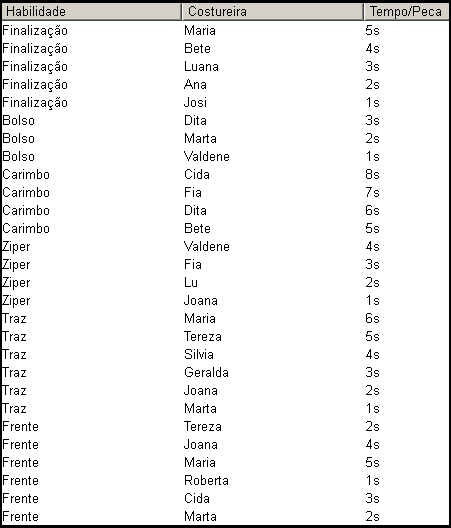
\includegraphics[width=10cm]{./imagens/tempo_habilidade2.png}}
	\caption[Costureiras e Habilidades]
	{Demonstração de costureiras e habilidades \textbf{Fonte:} Desenvolvido pelos autores}
	\label{fig:exemplo1}
\end{figure}


Uma costureira pode não receber nenhum lote (:0), isso permite que a decisão de quem vai participar ou não também 
fique por conta do algoritmo. O exemplo demonstrado está considerando que se irá produzir 500 peças em lotes de 50, 
resultando assim em um total de 10 lotes.

Feito esta distribuição será realizado um cálculo a fim de se encontrar o tempo total de fabricação do número de peças
desejado levando em consideração o tempo gasto por cada costureira para se produzir e o tempo gasto com o transporte 
das partes entre elas procurando assim encontrar uma forma de distribuir o trabalho de forma a se produzir as peças 
desejadas no menor tempo possível. Este cálculo será visto com mais detalhes na descrição do desenvolvimento da função 
de avaliação um pouco mais adiante.











\subsection{Desenvolvimento do Algoritmo genético}

\par 
As sessões abaixo descrevem como cada um destes elementos foram desenvolvidos no contexto do problema da fábrica de calças.




\subsubsection{Definição do indivíduo e Cromossomos}



\par Em um primeiro momento, o modelamento do indivíduo e seus cromossomos foi feito da seguinte forma:
Foi criado uma classe Java para representar o individuo denominada ProcessoIndividuo, esta classe é filha 
da classe Individual definida no framework. 

AINDA FALTA DESCREVER DUAS FORMAS QUE NAO DERAM CERTO


Todavia verificou-se que o algoritmo poderia apresentar problemas de performance. Um outro fator que 
influenciou para que se pensasse em uma nova abordagem foi o fato de somente parte da inteligência da distribuição
das horas ficarem sob responsabilidade do algoritmo, assim, sob a orientação do professor Artur Barbosa (mudar nome), 
o indivíduo e seus cromossomos foram desenvolvidos como descrito abaixo. Esta nova forma também facilitou o processo 
de cruzamento e mutação que será explanado mais adiante.

AINDA FALTA ESCREVER A FORMA QUE FOI FEITO (ESTAMOS ACABANDO A IMPLEMENTAÇÂO DESTA PARTE[Haja coração :(])

\subsubsection{Criação da população inicial}



\subsubsection{Desenvolvimento do mecanismo de Cruzamento e Mutação}



\subsubsection{Desenvolvimento da função de avaliação}
\par Conforme explicado na sessão que descreveu a classe \texttt{GAController}, a função de avaliação é chamada para se
avaliar cada indivíduo de uma nova população logo que esta é criada. A classe \texttt{ProcessoIndividual} é quem faz a 
implementação deste método.

\par Como descrito no escopo, após a distribuição dos lotes que foi feito aleatoriamente, foi desenvolvido
um algoritmo para fazer o cálculo para que se pudesse alcançar o tempo to tal de fabricação, levando em consideração 
o tempo gasto por cada costureira para se produzir e o tempo gasto com o transporte entre elas.  



 \begin{figure}[h!]
 	\centerline{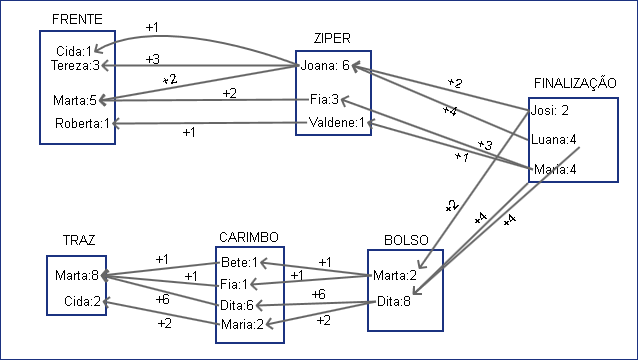
\includegraphics[scale=0.7]{./imagens/distribuicao_ilustracao.png}}
 	\caption[Distribuição de trabalho]
 	{Distribuição das atividades com precedência \textbf{Fonte:} Desenvolvido pelos autores}
 	\label{fig:exemplo1}
 \end{figure}
 
 \par O tempo gasto pela costureira é definido por \texttt{NLC * QPL * TP} em que \texttt{NLC} é o número de lotes atribuído
 para a costureira, \texttt{QPL} é a quantidade de peças por lote e o \texttt{TP} é o tempo que a costureira gasta para fazer
 cada peça, porém este tempo também é influenciado pelo tempo que se é gasto para receber as partes dependentes, veja na figura
 X:
 
\par No exemplo demonstrado na Figura X, em que está sendo considerado lotes de 50 peças, o algoritmo decidiu que 
a costureira Josi deverá fazer a atividade de Finalização de duas peças, assim como esta costureira gasta 2s para 
finalizar cada peça logo o tempo gasto para se produzir dois lotes será 2(NLC) * 50(QPL) * 2(TP), porém deve somar
a este resultado o tempo gasto para a Josi receber as peças da atividade predecessora, que neste caso é as peças 
da frente já com o Ziper.
\par A costureira Josi solicita então 2 lotes para as costureiras da atividade anterior começando pela Joana, a primeira
da lista que tem 6 lotes sob sua responsabilidade podendo assim ser aquela que irá enviar 2 lotes para a Joana, neste 
caso é feito então um cálculo de quanto tempo é gasto para a Joana realizar a atividade de colocar o Ziper em 2 lotes
 
Como algumas
atividades em alguns casos dependem de outras, pode ser que uma costureira para fazer 5 lotes por exemplo pegue 3 lotes da
costureira A e 2 lotes da costureira B da atividade anterior neste caso, as costureiras A e B da atividade anterior irão
precisar de 3 e 2 lotes respectivamente da atividade anterior e assim por diante, assim será considerado o maior tempo 
de fabricação e transporte para que cada costureira receba sua peça dependente. A Figura X ilustra este processo.

\par Como foi explicado no processo de desenvolvimento do mecanismo de cruzamento, um \texttt{ArrayList} foi definido para armazenar
os cromossomos do indivíduo.



\subsubsection{Construção da interface gráfica, \texttt{CRUD} e apresentação dos dados}


% \begin{itemize}

%	\item Fazer uma prova de conceito com algoritmos genéticos para eliminar
%	dúvidas cruciais sobre a viabilidade do projeto;
	  
%	\item Realizar a coleta dos requisitos com o gestor da empresa;
%	\par Descrever sobre os requisitos
	
%	\item Executar procedimentos referente à engenharia do software;
	
%	\subsection{Realzação da Modelagem da base de dados};
	
	
%	\item Codificar o projeto;
%	 Problemas encontrados no desenvolvimento

%	\item Realizar testes.
	 
 %\end{itemize}
 
% \par Realizando todos os passos descritos acima, teremos como resultado final o
 %projeto finalizado.




% \label{cap:quadroMetodologico}
% 
% \par Conteúdo do quadro metodológico. Perceba a forma que se coloca uma palavra entre aspas: o \LaTeX~oferece muita ``facilitade de formatação''.
% 
% Exemplo de código Java:
% 
% \begin{lstlisting} [style=custom_Java,caption={[Métodos da classe \texttt{FilmeBean}]{Métodos da classe \texttt{FilmeBean}. \textbf{Fonte:} Elaborado pelos autores.}}, label=fig:metodosclassebean] 	
% 	public FilmeBean(){  
%        //...
%    	}	
%    	
% 	public void saveMovie(){
% 		setListActorSelected();		
% 		if(this.movieDAO.saveMovieGraph(this.movieTo)){
% 			FacesContext.getCurrentInstance().addMessage(null, 
% 			   new FacesMessage("Filme cadastrado com sucesso!")); 
% 		}else{
% 			//...
% 		}		
% 		this.limpaCampos();
% 	}
% \end{lstlisting}
% 
% \par Agora será mostrado o exemplo do uso de fluxo de eventos apresentado no Quadro~\ref{quad:fluxo_evento_cadastro_filme}.
% 
% \begin{quadro}[h!]
%   \begin{fluxoDeEventos}
  \addTitle{Cadastrar filme}
  \addrow{Ator principal}{Administrador}
  %\addrow{Ator secundário}{Sistema de cartão}
  \addrow{Pré-requisitos}{Estar logado no sistema}

  \startBasicFlow{Ator} {Sistema}
  \addItemOne{Seleciona menu cadastro}
  \addItemOne{Clica na opção cadastrar filme}
  \addItemTwo{Abre interface de cadastro de filme}
  \addItemOne{Preenche formulário}
  \addItemOne{Clica no botão salvar}
  \addItemTwo{Salva e informa sucesso no cadastro}

  \startAlternativeFlow{Fluxo alternativo 1}
  \addItemOne{No item 5, formulário não preenchido}
  \addItemTwo{Exibe mensagem de necessidade de preenchimento de formulário}

  \startAlternativeFlow{Fluxo alternativo 2}
  \addItemOne{No item 6, inserido filme já cadastrado}
  \addItemTwo{Informa mensagem de filme já cadastrado}
\end{fluxoDeEventos}

%   \caption[Fluxo de eventos para cadastro de filme]
%            {Fluxo de eventos para cadastro de filme. \textbf{Fonte:} Elaborado pelos autores}
%   \label{quad:fluxo_evento_cadastro_filme}
% \end{quadro}
% 
% \par Outro exemplo é ilustrado na Figura~\ref{fig:bluesky}. Neste caso um código XML foi embutido dentro de um ambiente de figura, para que este código seja incluído no índice de figuras adequadamente.
%  
% \begin{figure}[ht!]
%   \begin{lstlisting} [style=custom_XML]
% 	...
% 	<context-param>
% 		<param-name>primefaces.THEME<\param-name>
% 		<param-value>bluesky<\param-value>
% 	<\context-param>
% 	...
%   \end{lstlisting}
%   \caption[Incluindo o tema \textit{BlueSky} ao contexto do projeto]
%           {Incluíndo o tema \textit{BlueSky} ao contexto do projeto. \textbf{Fonte:} Elaborado pelos autores.}
%   \label{fig:bluesky}
% \end{figure}
